\documentclass[11pt,a4paper]{article}
\usepackage[T1]{fontenc}
\usepackage[utf8]{inputenc}
\usepackage{lmodern}
\usepackage[margin=2.5cm]{geometry}
\usepackage{graphicx}
\usepackage{booktabs}
\usepackage{amsmath}
\usepackage{caption}
\usepackage{xcolor}
\usepackage[colorlinks=true,linkcolor=blue!50!black,urlcolor=blue!50!black,citecolor=blue!50!black]{hyperref}
\graphicspath{{figures/}}
\captionsetup{font=small,labelfont=bf}

\title{UFEM 2.0: Audit and Results of the Reinforced Concrete Beam\\Uncertainty Quantification Campaign}
\author{UFEM 2.0 Project}
\date{28 August 2026}

\begin{document}
\maketitle

\begin{abstract}
This report presents the audited results of a 400 sample Latin hypercube simulation campaign on a reinforced concrete beam modeled with concrete damaged plasticity in Abaqus. Of the 400 designed samples, 198 completed fully and 202 produced no output; the failure pattern is shown to be biased in the input space, so the surviving runs are a censored, non random subsample. Over the valid runs, the peak load is $38.15 \pm 3.49$~kN (coefficient of variation 9.2\,\%), the displacement at peak is $11.08 \pm 1.95$~mm, and the initial stiffness is $13.13 \pm 1.47$~kN/mm. Concrete strength dominates the peak load (Pearson $r = 0.80$), while the top reinforcement cover dominates the initial stiffness ($r = 0.50$). Two findings materially constrain any downstream surrogate model: the elastic modulus in the design is an exact deterministic function of the concrete strength (Spearman $\rho = 1.000$), so the campaign has three independent inputs rather than four; and the terminal compressive damage saturates at the material table cap of 0.947 in every single run, so it carries no information as a quantity of interest. This report is the Phase P2 deliverable of the UFEM~2.0 build specification and every number in it is regenerated by the audit pipeline from the raw extracted data.
\end{abstract}

\section{Introduction}
The UFEM project quantifies the effect of material and geometric uncertainty on the nonlinear response of a reinforced concrete member. A parametric Abaqus model was evaluated over a 400 point Latin hypercube design; the load displacement curve and a global damage evolution curve were extracted from each converged analysis. This document reports what the campaign actually produced, quantitatively and without retouching: the completion statistics and their bias, the response statistics over the valid runs, the input to output relations, and the consequences for surrogate construction. It replaces all previously circulated summary numbers for this campaign, which descended from a post processing chain with documented defects, including artificially injected variance in the uncertainty stage.

\section{The finite element model}
The member is a two dimensional plane stress idealization: a $2000 \times 250$~mm concrete domain of thickness 150~mm, meshed with 637 four node reduced integration elements, with two embedded truss reinforcement layers (three 10~mm bars near the bottom face, three 12~mm bars near the top face, perfect bond). The member is supported by a pin at $x = 200$~mm on the top edge and a roller at $x = 1000$~mm on the bottom edge, and is loaded by a prescribed vertical displacement of 20~mm at the tip of the 800~mm overhang, i.e.\ displacement control throughout, which is why every converged run spans the full displacement range. Concrete is modeled with the damaged plasticity formulation (dilation angle $30^\circ$, eccentricity 0.1, $f_{b0}/f_{c0} = 1.16$, $K = 0.667$, viscosity parameter $8 \times 10^{-4}$); the hardening, stiffening, and damage tables are scaled per sample from the sampled strength. Steel is elastic plastic (500~MPa yield, 520~MPa at 1.5\,\% plastic strain).

Two modeling limitations are inherited by every result in this report and are scheduled for correction in the follow up campaign: the tension softening definition is not regularized by fracture energy while the strength varies between samples, and no mesh convergence study was performed for the production mesh.

\section{Probabilistic model and design}
The design varies three independent random variables by Latin hypercube sampling (seed 42): the mean concrete compressive strength $f_{cm}$, lognormal with mean 28.0~MPa and coefficient of variation 0.10; the bottom cover $c_{\mathrm{bot}}$, normal with mean 27.0~mm and standard deviation 3.0~mm; and the top cover $c_{\mathrm{top}}$, normal with mean 223.0~mm and standard deviation 5.0~mm. The elastic modulus was generated as the Eurocode~2 expression $E = 22000\,(f_{cm}/10)^{0.3}$~MPa.

The audit verified this relation holds exactly in the design data: the maximum deviation between the stored $E$ and the expression above is $7.3 \times 10^{-12}$~MPa, and the rank correlation between $f_{cm}$ and $E$ is exactly one (Figure~\ref{fig:collinearity}). The campaign therefore has three independent inputs. Any regression or sensitivity analysis that treats $E$ as a fourth free input is ill posed: variance based indices split the shared effect arbitrarily between two copies of the same random variable. All analyses in this report, and the surrogate specified for the next phase, use the feature vector $(f_{cm}, c_{\mathrm{bot}}, c_{\mathrm{top}})$ only.

\begin{figure}[tbp]
\centering
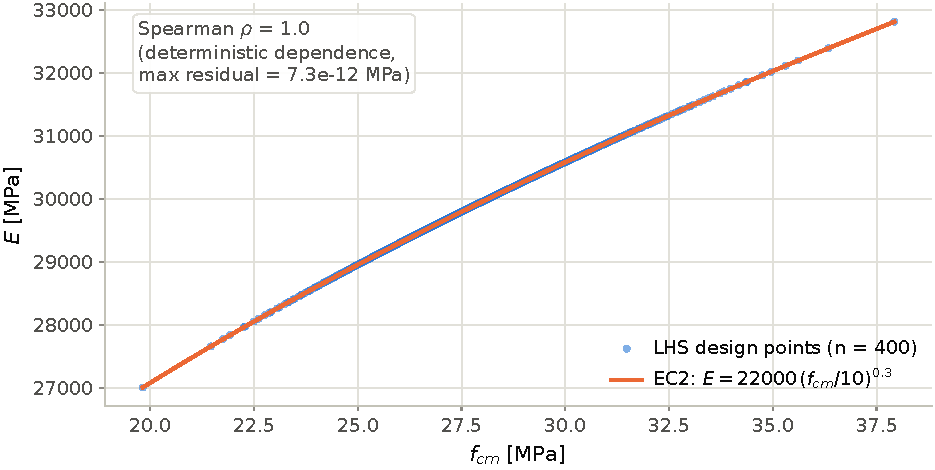
\includegraphics[width=0.72\linewidth]{fig_E_collinearity.pdf}
\caption{Elastic modulus against concrete strength for all 400 design points, with the Eurocode~2 curve overlaid. The stored modulus is an exact deterministic function of the strength (Spearman $\rho = 1.000$, maximum deviation $7.3\times10^{-12}$~MPa): the design has three independent inputs, not four.}
\label{fig:collinearity}
\end{figure}

\section{Campaign outcome and censoring}
\label{sec:censoring}
Of 400 designed samples, 198 completed and appear in the extracted data; 202 are absent entirely. There is no partial tier: every present run reached the final pseudo time exactly, captured a strictly interior load peak, and descended on the softening branch (post peak drop between 10\,\% and 78\,\% of peak, median 54\,\%), with no missing values and monotone displacement histories. The failure mode of this campaign is binary: an analysis either finished or left nothing.

The failures are not random in the input space (Figure~\ref{fig:censoring}). Failed samples have a lower mean top cover than completed ones (221.8 against 224.2~mm; Welch $p = 8\times10^{-7}$, chi squared over quartiles $p = 3\times10^{-11}$) and a higher mean strength (28.4 against 27.6~MPa, $p = 0.006$). Figure~\ref{fig:failrate} shows the failure rate by input quartile: the lowest top cover quartile fails at 76\,\%, the third quartile at 26\,\%, and the failure rate rises monotonically with strength from 38\,\% to 63\,\%. The bottom cover shows no significant effect ($p = 0.17$).

\begin{figure}[tbp]
\centering
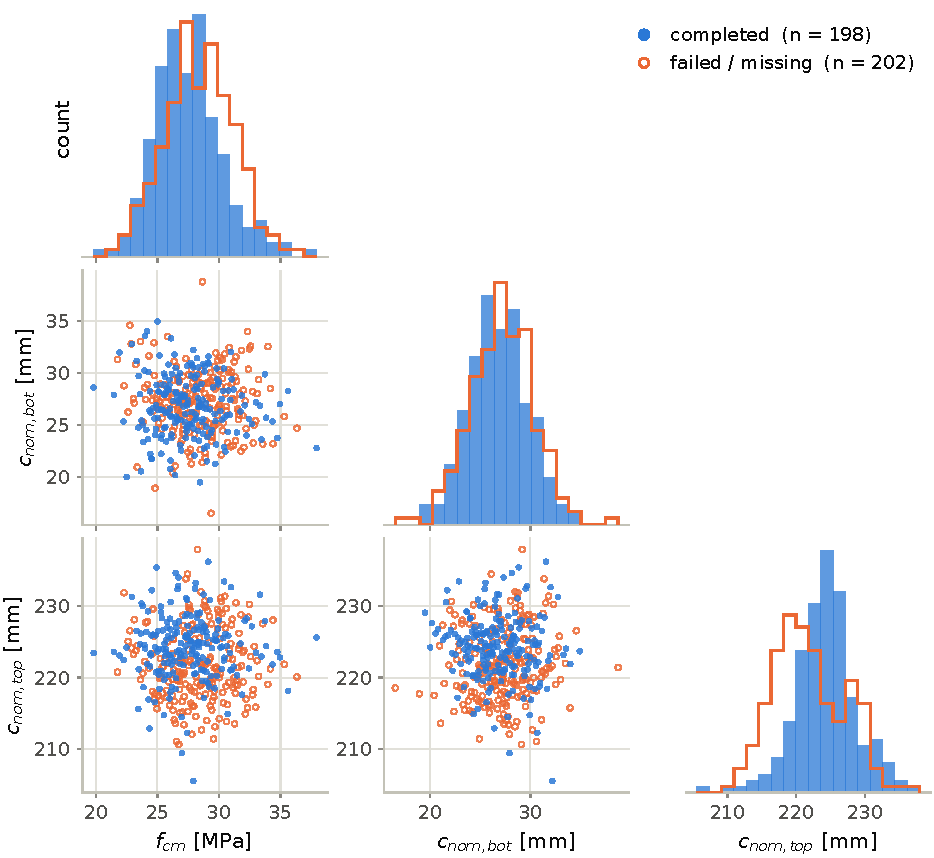
\includegraphics[width=0.9\linewidth]{fig_design_censoring.pdf}
\caption{The 400 point design projected on the three independent inputs, completed runs against failed runs. The surviving 198 runs are enriched in high top cover and low strength: a censored, biased subsample of the intended design.}
\label{fig:censoring}
\end{figure}

\begin{figure}[tbp]
\centering
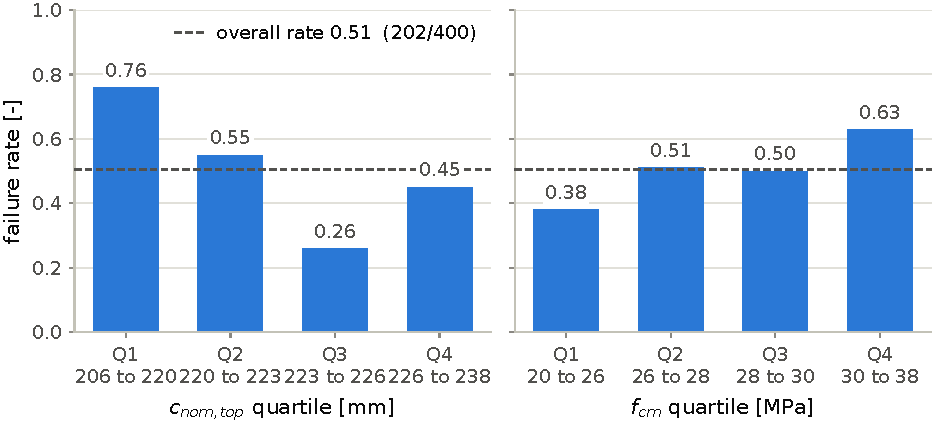
\includegraphics[width=0.9\linewidth]{fig_failure_rate_ctop.pdf}
\caption{Failure rate by input quartile ($n = 100$ per quartile). Left: top cover, failing at 76\,\% in the lowest quartile against 26\,\% in the third. Right: concrete strength, rising from 38\,\% to 63\,\% with increasing strength.}
\label{fig:failrate}
\end{figure}

Two consequences follow. First, every statistic in Section~\ref{sec:stats} is an estimate over a censored design, and population level claims inherit that bias; the effect is conservative for stiffness (the surviving set over represents stiff configurations) and of uncertain sign for the peak load. Second, any surrogate trained on the 198 valid runs has a validity domain: predictions in the low top cover, high strength corner extrapolate into a region where the solver itself predominantly failed, and the build specification requires that region to be flagged in every downstream product. The production solver logs are not preserved in the surviving tree, so the root cause of the 202 losses cannot be diagnosed retrospectively; re running the missing samples under the corrected model configuration is the stated first priority of the follow up campaign.

\section{Response statistics over the valid runs}
\label{sec:stats}
All 198 valid load displacement curves, interpolated onto a common 201 point displacement grid spanning 0 to 20~mm, are shown in Figure~\ref{fig:ldfamily}; the damage evolution family is shown in Figure~\ref{fig:damagefamily}. Table~\ref{tab:stats} summarizes the scalar quantities of interest.

\begin{figure}[tbp]
\centering
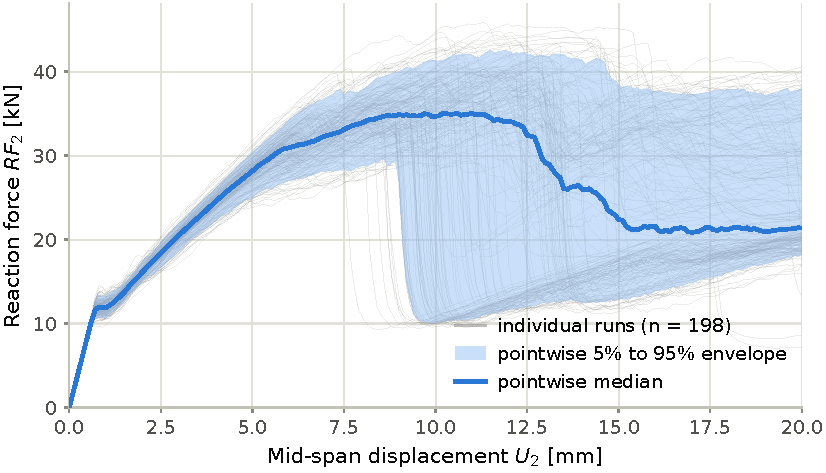
\includegraphics[width=0.85\linewidth]{fig_ld_family.pdf}
\caption{The 198 valid load displacement curves (thin lines), the pointwise median (bold), and the pointwise 5 to 95\,\% envelope (shaded). The median curve peaks at 35.0~kN at 10.2~mm; the envelope is widest, 31.6~kN, at 10.9~mm, where the curves disagree about the onset of softening.}
\label{fig:ldfamily}
\end{figure}

\begin{figure}[tbp]
\centering
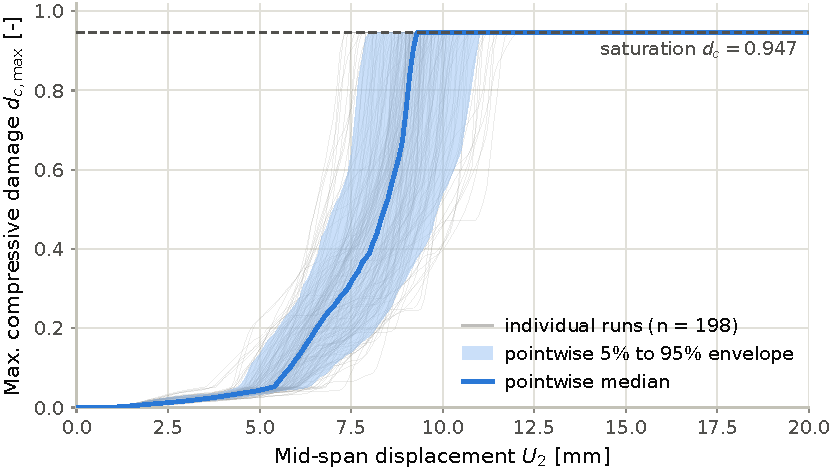
\includegraphics[width=0.85\linewidth]{fig_damage_family.pdf}
\caption{Compressive damage evolution for all 198 runs. Every run saturates at exactly 0.947, the cap of the material damage table, reached between roughly 7 and 12~mm of imposed displacement (median displacement at half saturation 8.35~mm). The terminal damage value carries zero variance and no information.}
\label{fig:damagefamily}
\end{figure}

\begin{table}[tbp]
\centering
\caption{Scalar quantities of interest over the 198 valid runs.}
\label{tab:stats}
\begin{tabular}{lrrrrr}
\toprule
Quantity & Mean & Std.\ dev. & CoV & Min & Max \\
\midrule
Peak load [kN] & 38.15 & 3.49 & 0.092 & 29.24 & 45.84 \\
Displacement at peak [mm] & 11.08 & 1.95 & 0.176 & 7.30 & 17.93 \\
Initial stiffness [kN/mm] & 13.13 & 1.47 & 0.112 & 9.50 & 17.33 \\
Residual load at 20 mm [kN] & 24.73 & 6.97 & 0.282 & 7.18 & 40.58 \\
Displacement at half damage saturation [mm] & 8.44 & 0.85 & 0.101 & 6.50 & 11.00 \\
Damage at 10 mm displacement & 0.886 & 0.140 & 0.158 & 0.396 & 0.947 \\
Terminal damage & 0.947 & 0.000 & 0.000 & 0.947 & 0.947 \\
\bottomrule
\end{tabular}
\end{table}

The peak load distribution (Figure~\ref{fig:peakstats}) is unimodal with 5 and 95\,\% quantiles at 32.3 and 43.4~kN. The scatter grows along the curve: the coefficient of variation rises from 11\,\% in the initial stiffness to 28\,\% in the residual load at 20~mm, i.e.\ the softening branch is where the input uncertainty expresses itself most strongly, and where a surrogate's calibration will be hardest to achieve.

The terminal damage row of Table~\ref{tab:stats} is the second structural finding of the audit: all 198 runs end at the same value, 0.947, which is the float32 image of the compression damage table cap. Any analysis that propagates terminal damage, or defines a failure threshold above 0.947, is vacuous by construction; the informative damage descriptors are the displacement at half saturation and the damage at a fixed intermediate displacement, both of which vary substantially between runs.

\begin{figure}[tbp]
\centering
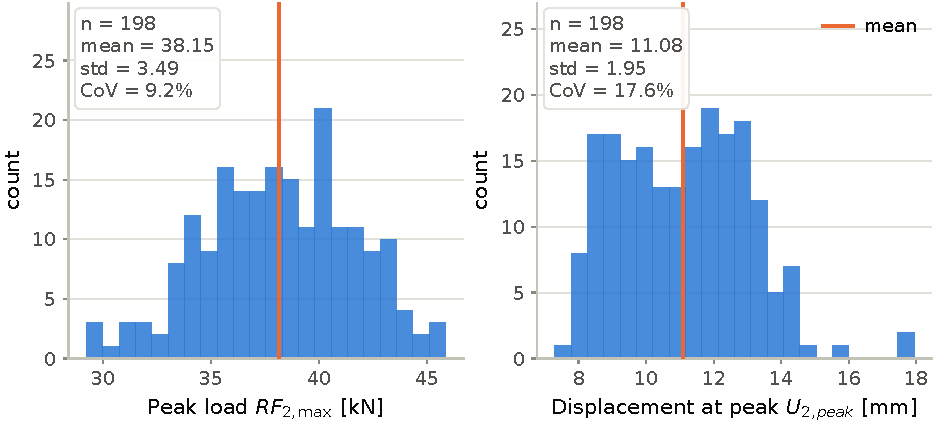
\includegraphics[width=0.9\linewidth]{fig_peak_stats.pdf}
\caption{Distributions over the 198 valid runs of the peak load (left; mean 38.15~kN, CoV 9.2\,\%) and the displacement at peak (right; mean 11.08~mm, CoV 17.6\,\%).}
\label{fig:peakstats}
\end{figure}

\section{Input to output relations}
Figure~\ref{fig:peakvsinputs} shows the peak load against each independent input. Concrete strength dominates ($r = 0.80$; the rank correlation is 0.81), the top cover contributes a secondary positive effect ($r = 0.24$), and the bottom cover a weak negative one ($r = -0.14$). The initial stiffness tells a different story (Figure~\ref{fig:stiffness}): it is governed primarily by the top cover ($r = 0.50$), with strength contributing only weakly through the modulus ($r = 0.13$). The displacement at peak correlates negatively with top cover ($r = -0.38$) and positively with strength ($r = 0.27$), and the damage at 10~mm correlates negatively with strength ($r = -0.46$): stronger concrete both raises the peak and delays damage accumulation.

These monotone, smooth, moderately interacting relations over three inputs are exactly the regime in which Gaussian process surrogates on a reduced curve representation are expected to perform well, and in which a linear baseline already explains a substantial fraction of the peak load variance; the build specification therefore requires any surrogate to demonstrate out of sample superiority over that baseline rather than assume it.

\begin{figure}[tbp]
\centering
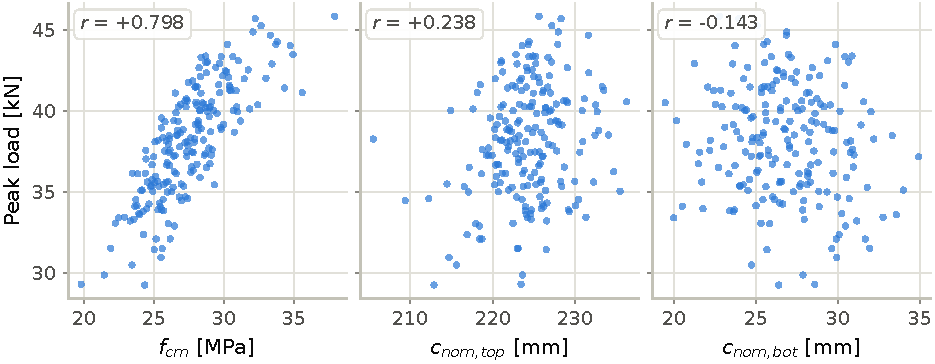
\includegraphics[width=\linewidth]{fig_peak_vs_inputs.pdf}
\caption{Peak load against the three independent inputs over the 198 valid runs, with Pearson correlations: strength dominates ($r = 0.80$), top cover is secondary ($r = 0.24$), bottom cover weak ($r = -0.14$).}
\label{fig:peakvsinputs}
\end{figure}

\begin{figure}[tbp]
\centering
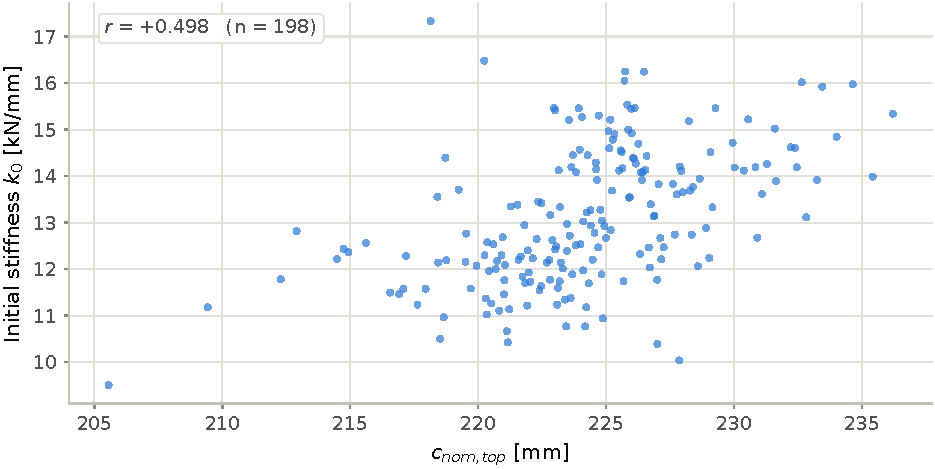
\includegraphics[width=0.62\linewidth]{fig_stiffness_vs_ctop.pdf}
\caption{Initial stiffness against top cover ($r = 0.50$): the geometric input, not the material strength, governs the elastic response.}
\label{fig:stiffness}
\end{figure}

\section{Consequences for surrogate construction}
The audit fixes five requirements for the surrogate phase. First, the common displacement grid is legitimate: because loading is displacement controlled, every valid curve spans exactly 0 to 20~mm, and interpolation onto a shared 201 point grid loses nothing (the coarsest native curve has 4854 points). Second, duplicated solver cutback time stamps occur in 26 of the 198 jobs and must be removed by a strict monotonicity filter before interpolation. Third, the feature vector is three dimensional; the modulus is derived, never regressed on. Fourth, the displacement at peak varies by a factor of 2.5 across the family, so the curves exhibit phase variability as well as amplitude variability, and a registration step before dimensionality reduction is required to avoid the known artifacts of principal component analysis on misaligned peaked curves. Fifth, every product downstream of the surrogate must carry the censoring caveat of Section~\ref{sec:censoring}.

\section{Conclusion}
The campaign delivered 198 fully converged, softening resolved load displacement and damage histories over a three dimensional input space, with clean, information rich response statistics: peak load CoV 9.2\,\%, growing to 28\,\% on the softening branch, strength controlled capacity, and cover controlled stiffness. It also delivered two hard lessons that the successor pipeline is built around: half the design was lost to a biased, undiagnosed failure mode, and two of the nominal outputs (the fourth input and the terminal damage) carry no independent information at all. Every number in this report is regenerated by the audit stage of the UFEM~2.0 pipeline from the raw extracted CSV files; the audit script, the validity classification of all 400 samples, and the machine readable summary are archived alongside this document.

\end{document}
